\documentclass{beamer}

\usepackage[utf8]{inputenc}
\graphicspath{{../Graphics/}}

%Information to be included in the title page:
\title{Heat Energy Sources in Canada}
\author{Noah Bolohan, Anton Iatcenko, Ryan Thiessen, Yakine Bahri, Benjamin MacAdam, Alireza Yazdani}
\institute{Math\textsuperscript{Industry}}

\date{August 2020  \\ \vspace{30pt} 
\includegraphics[scale=0.3]{pims_logo.png} }



\begin{document}

\frame{\titlepage}

\begin{frame}
\frametitle{The Data Set (Yakine)}
\textbf{Primary heating systems and type of energy} : A table contains 2304 series, with data for years 2013, 2015 and 2017
It contains data described by the following dimensions:
\begin{itemize}
\item Geography (48 items: Canada; Newfoundland and Labrador; Prince Edward Island; Nova Scotia; ...)
\item Primary heating system and type of energy (48 items: All primary heating systems; Electricity; Natural gas; Oil; ...).
\end{itemize}
\textbf{Source} : https://open.canada.ca/data/en/dataset/ec3282b6-013f-41b1-aa63-24ad8bda79ee
\end{frame}


\begin{frame}
\frametitle{Primary heating types in Canada: 2013-2017}
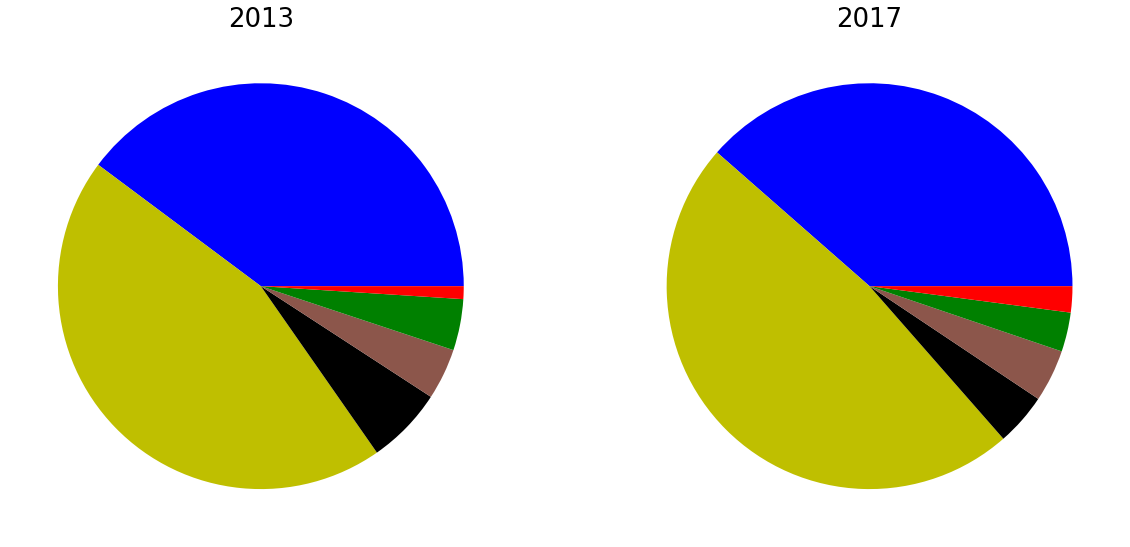
\includegraphics[width=\textwidth]{Canada20132017.png}\\
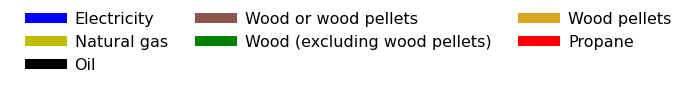
\includegraphics[width=\linewidth]{leg_bar.png}
\end{frame}



\begin{frame}
\frametitle{Change Over Time I (Anton)}
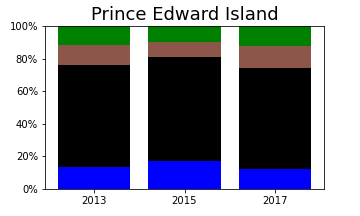
\includegraphics[width=0.5\linewidth]{pe.png}%
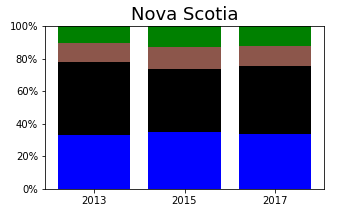
\includegraphics[width=0.5\linewidth]{ns.png}\\
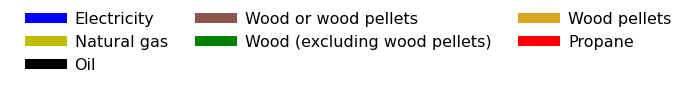
\includegraphics[width=\linewidth]{leg_bar.png}
\end{frame}


\begin{frame}
\frametitle{Change Over Time II (Anton)}
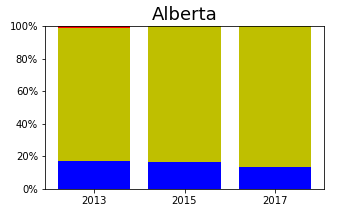
\includegraphics[width=0.5\linewidth]{ab.png}%
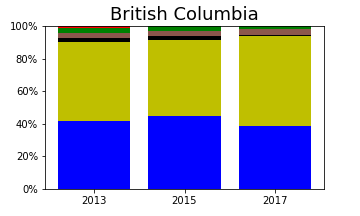
\includegraphics[width=0.5\linewidth]{bc.png}\\
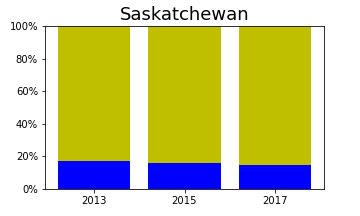
\includegraphics[width=0.5\linewidth]{sk.png}%
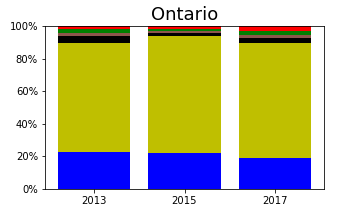
\includegraphics[width=0.5\linewidth]{on.png}\\
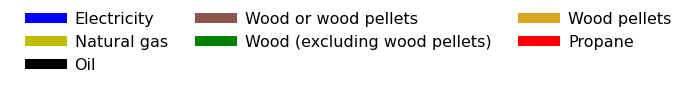
\includegraphics[width=\linewidth]{leg_bar.png}
\end{frame}


\begin{frame}
\frametitle{Change Over Time III (Anton)}
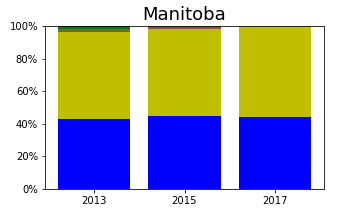
\includegraphics[width=0.5\linewidth]{mn.png}%
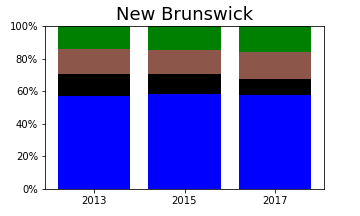
\includegraphics[width=0.5\linewidth]{nb.png}\\
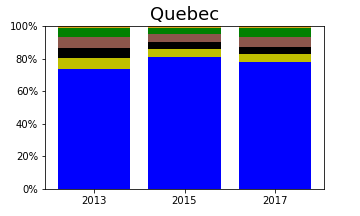
\includegraphics[width=0.5\linewidth]{qc.png}%
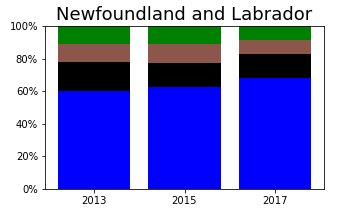
\includegraphics[width=0.5\linewidth]{nl.png}\\
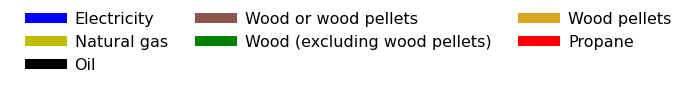
\includegraphics[width=\linewidth]{leg_bar.png}
\end{frame}



\begin{frame}
\frametitle{Province Groupings (Anton)}


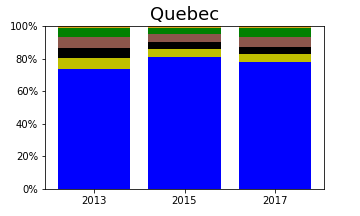
\includegraphics[width=0.33\linewidth]{qc.png}%
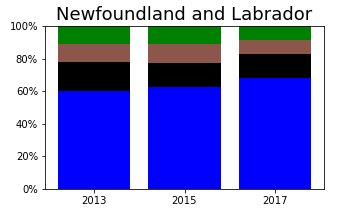
\includegraphics[width=0.33\linewidth]{nl.png}%
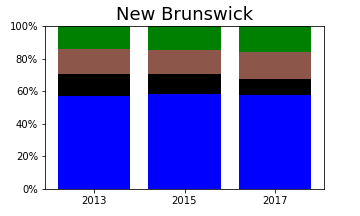
\includegraphics[width=0.33\linewidth]{nb.png}\\[10pt]
%
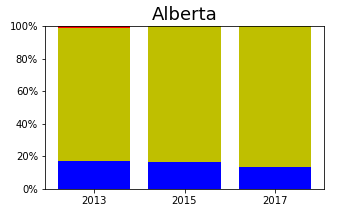
\includegraphics[width=0.33\linewidth]{ab.png}%
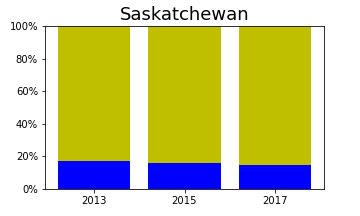
\includegraphics[width=0.33\linewidth]{sk.png}%
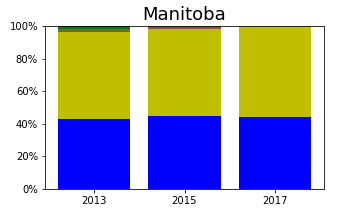
\includegraphics[width=0.33\linewidth]{mn.png}\\[10pt]
%
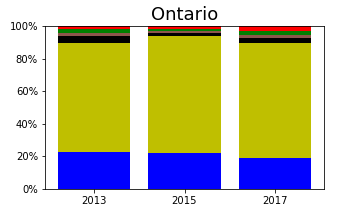
\includegraphics[width=0.25\linewidth]{on.png}%
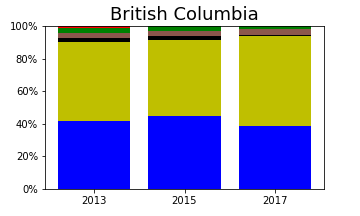
\includegraphics[width=0.25\linewidth]{bc.png}%
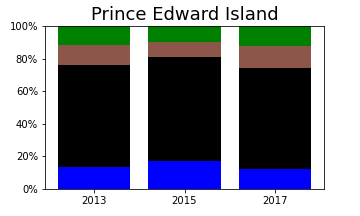
\includegraphics[width=0.25\linewidth]{pe.png}%
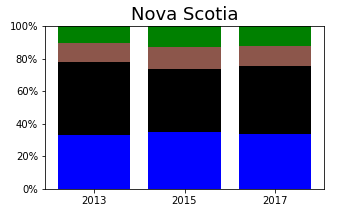
\includegraphics[width=0.25\linewidth]{ns.png}


\end{frame}


\begin{frame}

\frametitle{Cause of the Groupings: Natural Gas}

\begin{center}
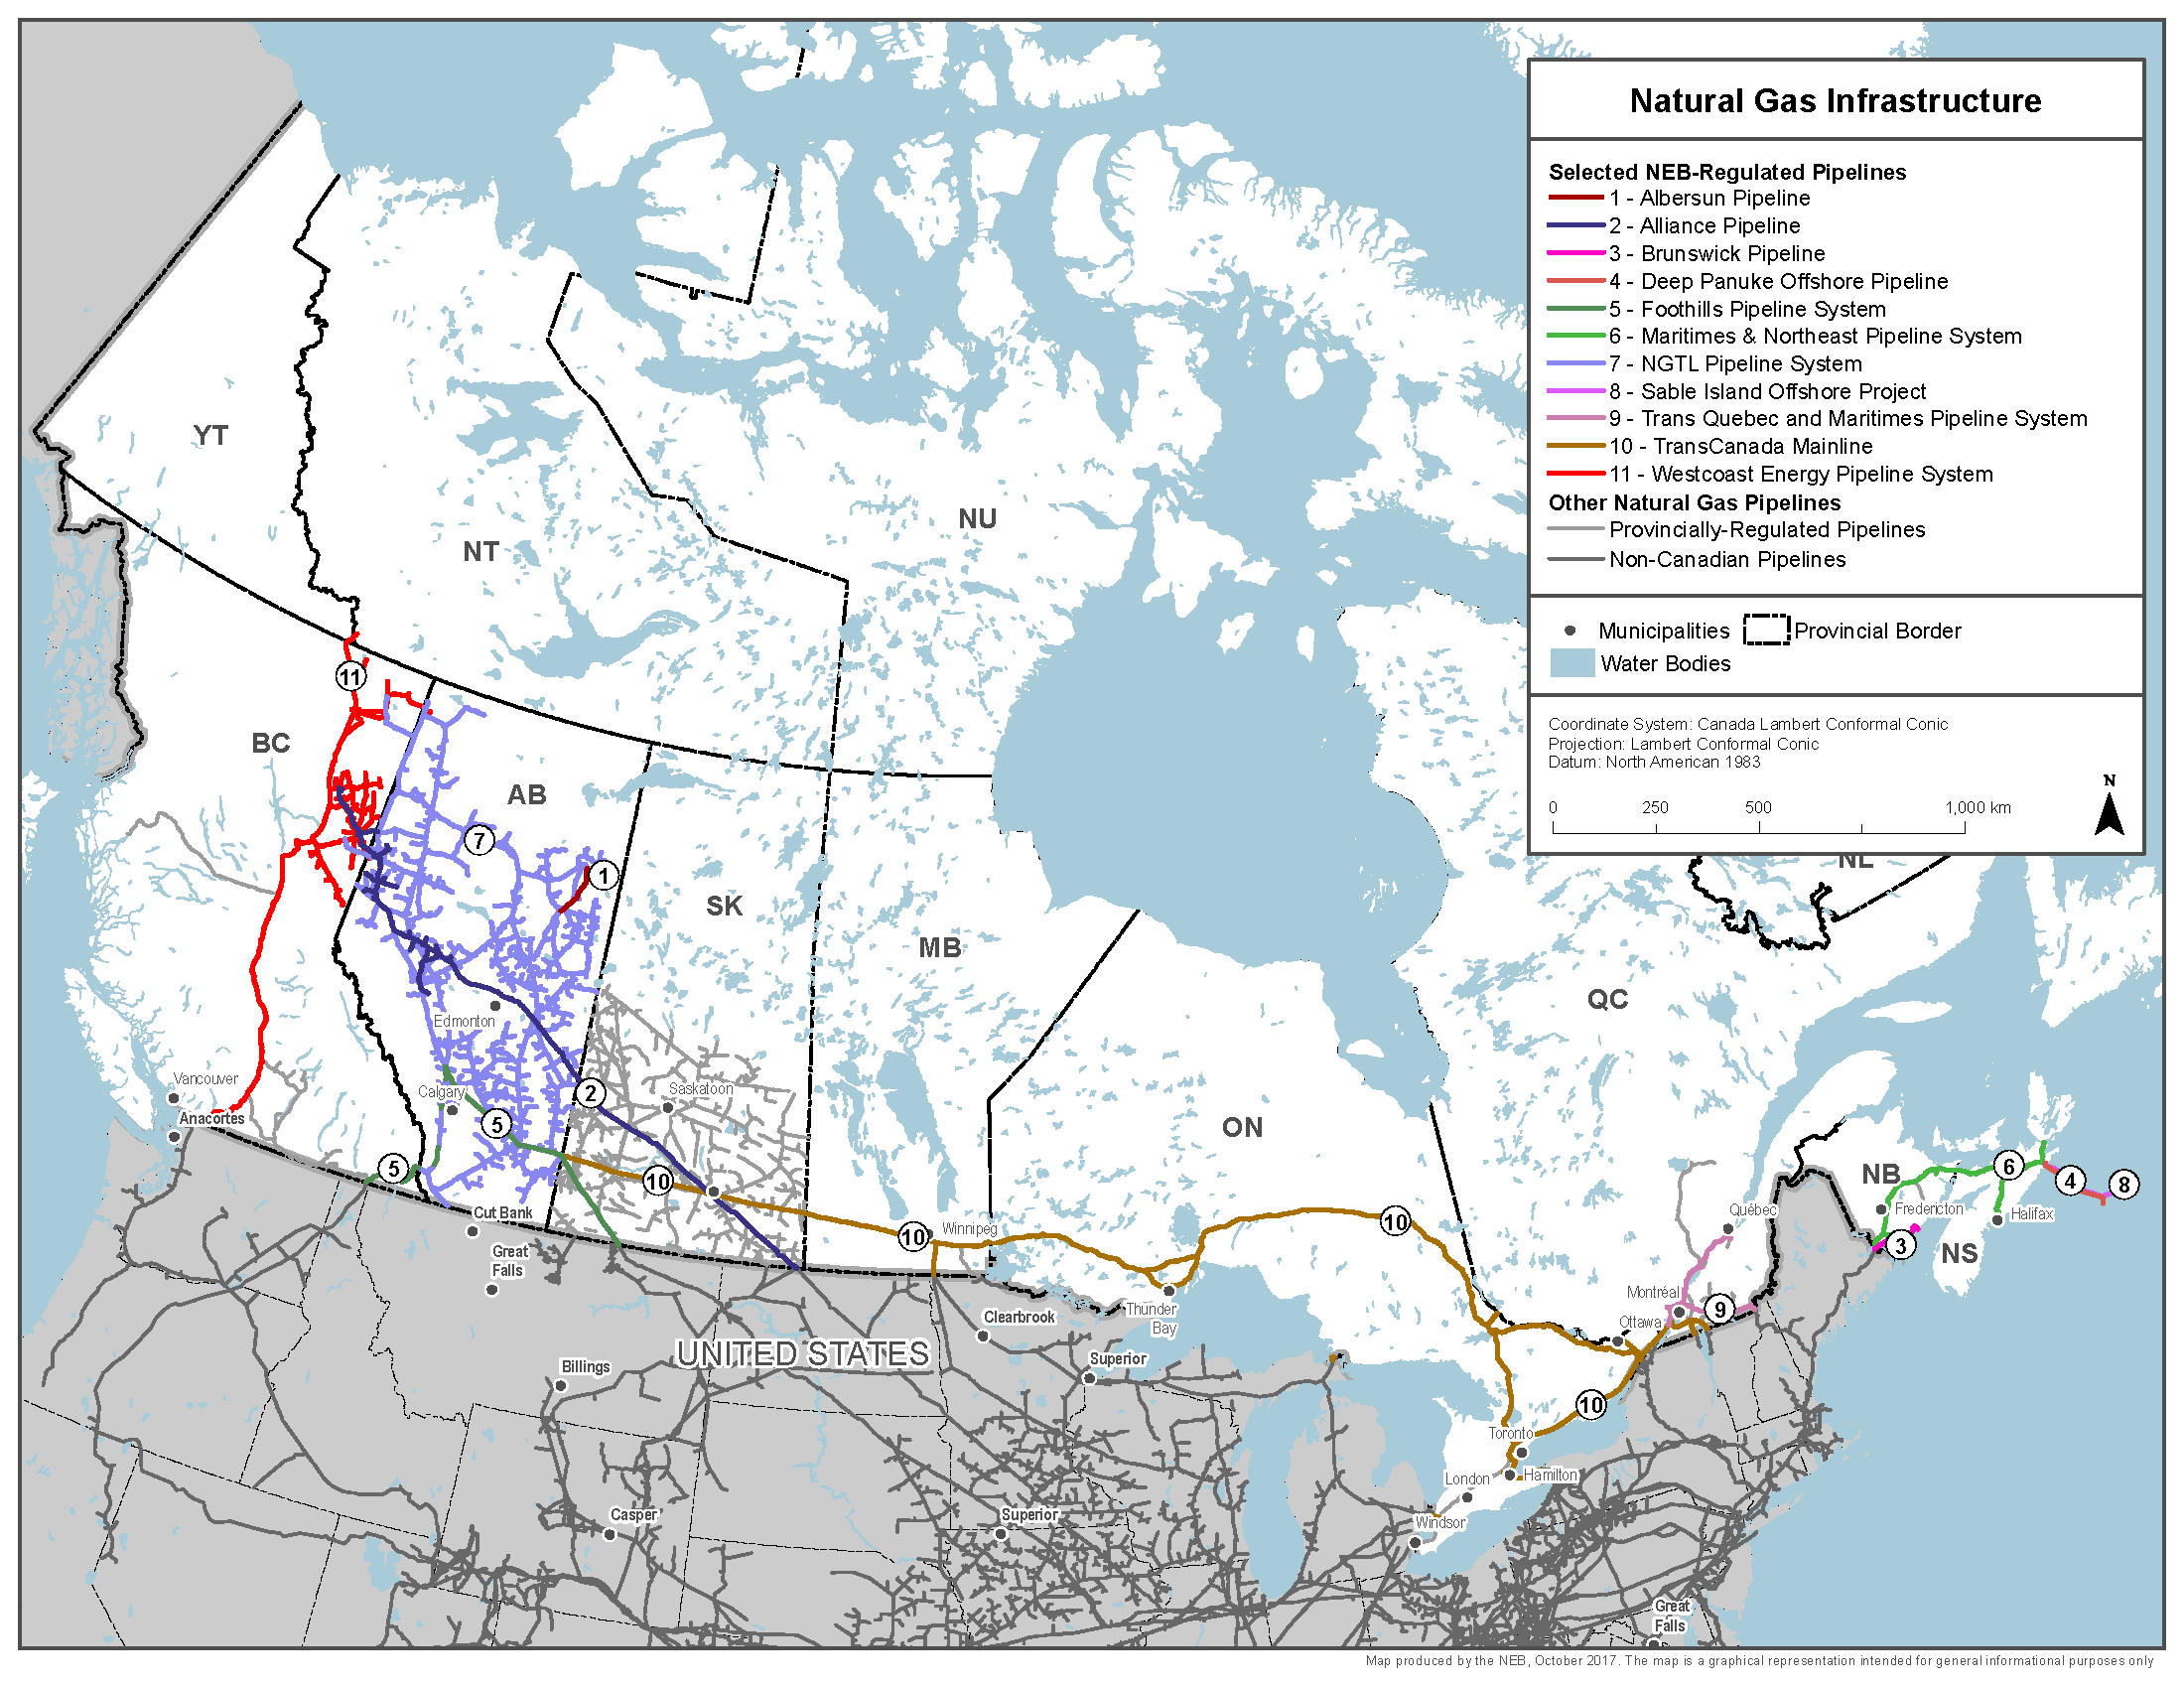
\includegraphics[width=0.6\textwidth]{natural_gas_pipeline_natural_resources_canada}
\end{center}
\vspace{-10pt}

\small
\begin{itemize}
	\item SK, AB, and parts of BC have an extensive natural gas infrastructure.
	\item MB and ON have access to the natural gas TransCanada pipeline.
\end{itemize}
\normalsize
\end{frame}


\begin{frame}
\frametitle{Cause of the Groupings: Electricity (Alireza)}

\end{frame}


\begin{frame}
\frametitle{Cause of the Groupings: Atlantic Provinces (Ben)}

	\begin{tabular}{ c c}
	  \scalebox{0.3}{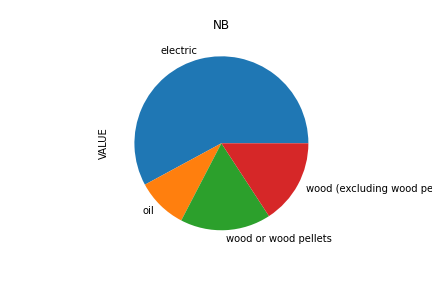
\includegraphics{Ben_Images/NB.png}}
	& \scalebox{0.3}{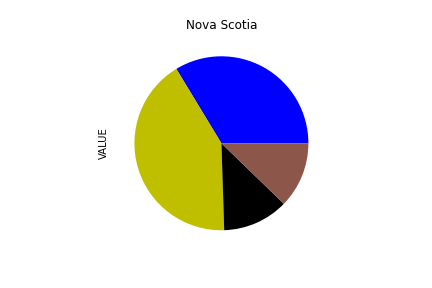
\includegraphics{Ben_Images/NS.png}} \\
	\scalebox{0.3}{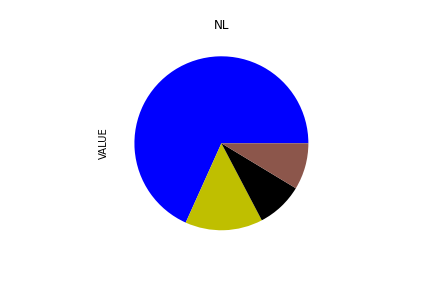
\includegraphics{Ben_Images/NL.png}}
	& \scalebox{0.3}{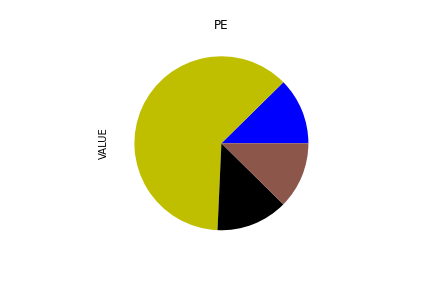
\includegraphics{Ben_Images/PE.png}}
	\end{tabular}
	Same story in Atlantic region:
	\begin{itemize}
		\item NL,NB: Access to hydro, use electric.
		\item PE, NS: No access to Hydro, use oil.
	\end{itemize}
\end{frame}


\begin{frame}
\frametitle{Summary}

No change over time.

The dependence is predominantly geographic.

Thanks for your attention.

\end{frame}













\end{document}
